\documentclass[11pt, reqno]{amsart}
\usepackage[margin=1in]{geometry}    
\geometry{letterpaper}       
%\geometry{landscape}                % Activate for for rotated page geometry
\usepackage[parfill]{parskip}    % Deactivate to begin paragraphs with an indent rather than an empty line
\usepackage{amsfonts, amscd, amssymb, amsthm, amsmath}
\usepackage{pdfsync}  %leaves makers for tex searching
\usepackage{enumerate}
\usepackage{multicol}
\usepackage[pdftex,bookmarks]{hyperref}
\usepackage{enumitem}


\setlength\parindent{0pt}

%%% Theorems %%%--------------------------------------------------------- 
\theoremstyle{plain}
	\newtheorem{thm}{Theorem}[section]
	\newtheorem{lemma}[thm]{Lemma}
	\newtheorem{prop}[thm]{Proposition}
	\newtheorem{cor}[thm]{Corollary}
\theoremstyle{definition}
	\newtheorem*{defn}{Definition}
	\newtheorem{remark}{Remark}
\theoremstyle{example}
	\newtheorem*{example}{Example}


%%% Environments %%%--------------------------------------------------------- 
\newenvironment{ans}{\color{black}\medskip \paragraph*{\emph{Answer}.}}{\hfill \break  $~\!\!$ \dotfill \medskip }
\newenvironment{sketch}{\medskip \paragraph*{\emph{Proof sketch}.}}{ \medskip }
\newenvironment{summary}{\medskip \paragraph*{\emph{Summary}.}}{  \hfill \break  \rule{1.5cm}{0.4pt} \medskip }
\newcommand\Ans[1]{\color{black}\hfill \emph{Answer:} {#1}}


%%% Pictures %%%--------------------------------------------------------- 
%%% If you need to draw pictures, tikzpicture is one good option. Here are some basic things I always use:
\usepackage{tikz}
\usetikzlibrary{arrows}
\tikzstyle{V}=[draw, fill =black, circle, inner sep=0pt, minimum size=2pt]
\newcommand\TikZ[1]{\begin{matrix}\begin{tikzpicture}#1\end{tikzpicture}\end{matrix}}



%%% Color  %%%---------------------------------------------------------
\usepackage{color}
\newcommand{\blue}[1]{{\color{blue}#1}}
\newcommand{\NOTE}[1]{{\color{blue}#1}}
\newcommand{\MOVED}[1]{{\color{gray}#1}}


%%% Alphabets %%%---------------------------------------------------------
%%% Some shortcuts for my commonly used special alphabets and characters.
\def\cA{\mathcal{A}}\def\cB{\mathcal{B}}\def\cC{\mathcal{C}}\def\cD{\mathcal{D}}\def\cE{\mathcal{E}}\def\cF{\mathcal{F}}\def\cG{\mathcal{G}}\def\cH{\mathcal{H}}\def\cI{\mathcal{I}}\def\cJ{\mathcal{J}}\def\cK{\mathcal{K}}\def\cL{\mathcal{L}}\def\cM{\mathcal{M}}\def\cN{\mathcal{N}}\def\cO{\mathcal{O}}\def\cP{\mathcal{P}}\def\cQ{\mathcal{Q}}\def\cR{\mathcal{R}}\def\cS{\mathcal{S}}\def\cT{\mathcal{T}}\def\cU{\mathcal{U}}\def\cV{\mathcal{V}}\def\cW{\mathcal{W}}\def\cX{\mathcal{X}}\def\cY{\mathcal{Y}}\def\cZ{\mathcal{Z}}

\def\AA{\mathbb{A}} \def\BB{\mathbb{B}} \def\CC{\mathbb{C}} \def\DD{\mathbb{D}} \def\EE{\mathbb{E}} \def\FF{\mathbb{F}} \def\GG{\mathbb{G}} \def\HH{\mathbb{H}} \def\II{\mathbb{I}} \def\JJ{\mathbb{J}} \def\KK{\mathbb{K}} \def\LL{\mathbb{L}} \def\MM{\mathbb{M}} \def\NN{\mathbb{N}} \def\OO{\mathbb{O}} \def\PP{\mathbb{P}} \def\QQ{\mathbb{Q}} \def\RR{\mathbb{R}} \def\SS{\mathbb{S}} \def\TT{\mathbb{T}} \def\UU{\mathbb{U}} \def\VV{\mathbb{V}} \def\WW{\mathbb{W}} \def\XX{\mathbb{X}} \def\YY{\mathbb{Y}} \def\ZZ{\mathbb{Z}}  

\def\fa{\mathfrak{a}} \def\fb{\mathfrak{b}} \def\fc{\mathfrak{c}} \def\fd{\mathfrak{d}} \def\fe{\mathfrak{e}} \def\ff{\mathfrak{f}} \def\fg{\mathfrak{g}} \def\fh{\mathfrak{h}} \def\fj{\mathfrak{j}} \def\fk{\mathfrak{k}} \def\fl{\mathfrak{l}} \def\fm{\mathfrak{m}} \def\fn{\mathfrak{n}} \def\fo{\mathfrak{o}} \def\fp{\mathfrak{p}} \def\fq{\mathfrak{q}} \def\fr{\mathfrak{r}} \def\fs{\mathfrak{s}} \def\ft{\mathfrak{t}} \def\fu{\mathfrak{u}} \def\fv{\mathfrak{v}} \def\fw{\mathfrak{w}} \def\fx{\mathfrak{x}} \def\fy{\mathfrak{y}} \def\fz{\mathfrak{z}}
\def\fgl{\mathfrak{gl}}  \def\fsl{\mathfrak{sl}}  \def\fso{\mathfrak{so}}  \def\fsp{\mathfrak{sp}}  
\def\GL{\mathrm{GL}} \def\SL{\mathrm{SL}}  \def\SP{\mathrm{SL}}

\def\<{\langle} \def\>{\rangle}
\usepackage{mathabx}
\def\acts{\lefttorightarrow}
\def\ad{\mathrm{ad}} 
\def\Aut{\mathrm{Aut}}
\def\Ann{\mathrm{Ann}}
\def\dim{\mathrm{dim}} 
\def\End{\mathrm{End}} 
\def\ev{\mathrm{ev}} 
\def\Fr{\mathcal{F}\mathrm{r}}
\def\half{\hbox{$\frac12$}}
\def\Hom{\mathrm{Hom}} 
\def\id{\mathrm{id}} 
\def\sgn{\mathrm{sgn}}  
\def\supp{\mathrm{supp}}  
\def\Tor{\mathrm{Tor}}
\def\tr{\mathrm{tr}} 
\def\vep{\varepsilon}
\def\f{\varphi}


\def\Obj{\mathrm{Obj}}
\def\normeq{\unlhd}
\def\Set{{\cS\mathrm{et}}}
\def\Fin{{\cF\mathrm{inSet}}}
\def\Set{{\cS\mathrm{et}}}
\def\Grp{{\cG\mathrm{rp}}}
\def\Ab{{\cA\mathrm{b}}}
\def\Mod{{\cM\mathrm{od}}}
\def\ab{\mathrm{ab}}
\def\lcm{\mathrm{lcm}}
\def\ZZn{\ZZ/n\ZZ}


%%%%%%%%%%%%%%%%%%%%%%%%%%%%%% 
%%%%%%%%%%%%%%%%%%%%%%%%%%%%%%

\def\HW{5}
\def\DUE{10/27/2020}

\title[Homework \HW]{Homework \HW \\
Math A4900/44900\\
\small Due: \DUE}
\author{}

\begin{document}
%\maketitle %%% COMMENT THIS LINE OUT (add a % to the beginning of the line) and UNCOMMENT the following (delete the % symbols) to give yourself a good assignment header:
\begin{flushright}
Chris Hayduk\\
Math A4900\\
Course Summary\\
\DUE
\end{flushright}

\section{Introduction}

Algebra has been a prominent field of study within mathematics for thousands of years. Its origins date back to the Babylonians of the 1st millennium BCE, who used formulas to solve problems which were typically solved geometrically in other civilizations of the time \cite{algebrawiki}. The algebraic concepts introduced in Babylonia continued to be developed in Greece, India, and the the Islamic world over the next two thousand years \cite{algebrawiki}. During the Renaissance, much interest was given to the solutions of polynomial equations, with general solutions found for quadratic, cubic, and quartic polynomials \cite{pinter, algebrawiki}. However, solutions for quintic polynomials eluded mathematicians for centuries after this \cite{pinter, algebrawiki}.

\par
This push towards a general solution for quintic polynomials culminated in significant developments from Neils Abel and Évariste Galois in the 19th century \cite{pinter, algebrawiki}. After hundreds of years of searching for a general solution for quintic polynomials, in 1824 Abel showed that no such solution exists \cite{pinter}. Meanwhile in France, Évariste Galois pushed this result even further, developing what we now know as Galois Theory in order to answer the question: which polynomials of degree 5 or higher have solutions? \cite{pinter}. His results were published in 1847, 15 years after his untimely death, and represented a significant departure from the work of previous algebraists. While previous scholars viewed algebra as the theory of equations, it began to become clear that algebra could be defined in a much more general sense \cite{pinter, algebrawiki, abstractwiki}. Algebra gradually tended towards this more general, axiomatic approach until in 1930, Bartel van der Waerden published \textit{Moderne algebra}. This two-volume book synthesized the advances in algebra over the past century and thus formed the basis for today's ``modern algebra'' \cite{abstractwiki}. Hence, this book demarcated the change in algebra ``from the theory of equations to the theory of algebraic structures'' \cite{abstractwiki}.

\par
With this historical context in mind, we now turn our attention to studying this theory of algebraic structures. We start by examining groups, an algebraic structure which forms the foundation of much of algebra \cite{dummit, pinter}. Our foray into algebraic structures begins by examining the properties that arise from groups and their axioms. We learn about subgroups, which allow us to characterize subsets of groups which retain the group structure \cite{dummit, pinter, carter}. We then move onto homorphisms and isomorphisms. These functions and their properties aid us in talking about similarities between groups \cite{dummit}. In particular, homomorphisms allow us to describe the notion of quotient groups, which describes the group that is yielded when dividing a group by one of its normal subgroups \cite{dummit, carter}. We then examine group actions, in which we allow a group to act on a set \cite{dummit}. The properties of the set and the action on this set can inform us of the group's properties, and this forms a fundamental part of Galois Theory \cite{dummit}. Lastly, we switch gears to rings, which provide an extension of the material we learn about in regards to groups.

\newpage

\section{Topics}

\subsection{Groups}

\par
As mentioned in our introduction, groups are foundational to the modern study of algebra \cite{dummit, abstractwiki}. Groups are a quite general notion of an algebraic structure, consisting simply of a set with a binary operation on this set \cite{groupwiki}. Informally, a group consists of a set of elements and a method for combining those elements into new elements contained within the set \cite{pinter, carter}. We can visualize the concept of a basic group using a Rubik's cube, as shown in \textit{Visual Group Theory} \cite[\S 1.1, p. 4]{carter}:

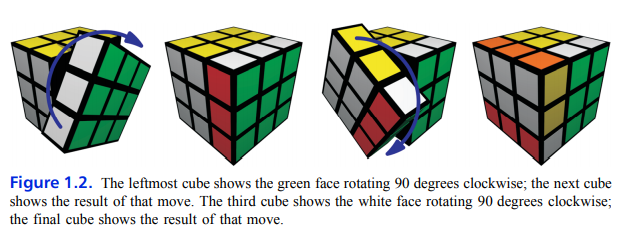
\includegraphics[scale=1]{rubiks}

\par
The cube provides a set of elements, namely any possible move that we can apply to the Rubik's cube. In addition, we see that we can combine actions in order to yield a new possible action within the set. For example, two $90^{\circ}$ rotations of a particular face will yield a $180^{\circ}$ rotation of that face. Moreover, the reverse rotation can be made so that we return to the original cube configuration \cite{carter}. Hence, we see that we can combine moves to form new, valid moves and that each valid move has a reverse move on the cube. This provides an intuitive notion of a group and its structure.

\par
Another clear and intuitive example of a group structure is given by the dihedral group, which describes the rotations and reflections of a regular polygon \cite{dummit, dihedralwiki}. We can see a visual example of the $D_8$, the dihedral group on a polygon with $8$ sides, by looking at the rotations and reflections of a stop sign \cite{dihedralwiki}:

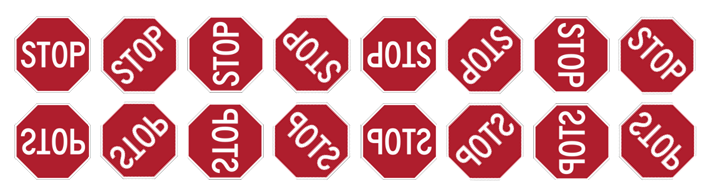
\includegraphics[scale=0.65]{Dihedral8}

Each rotation and reflection changes the configuration of our stop sign, and we can combine these rotations and reflections in order to yield even more new configurations. In total, we have that there are $16$ unique moves that we can on the stop sign make by taking any possible sequence of rotations and reflections \cite{dihedralwiki}.

\newpage
\par
Now that we have an intuitive sense of what groups are and how they work, let us formally define what a group is \cite[\S 1.1, p. 16]{dummit}:

\par
\textbf{Definition}
\begin{enumerate}
\item A \textit{group} is an ordered pair $(G, *)$ where $G$ is a set and $*$ is a binary operation on $G$ satisfying the following axioms:

\begin{enumerate}[label=(\roman*)]
\item $(a * b) * c = a * (b * c)$, for all $a, b, c \in G$, i.e. $*$ is \textit{associative}

\item there exists an element $e$ in $G$ called an \textit{identity} of $G$, such that for all $a \in G$, we have $a * e = e * a = a$

\item for each $a \in G$ there is an element $a^{-1}$ of $G$ called an \textit{inverse} of $a$ such that $a * a^{-1} = a^{-1} * a = e$

\end{enumerate}

\item The group $(G, *)$ is called \textit{abelian} (or \textit{commutative}) if $a * b = b * a$ for all $a, b \in G$.
\end{enumerate}

$(1)$ in the above definition provides a formalization of the intuitive notion of groups that we introduced with the Rubik's cube and dihedral groups. We see that grouping of operations on elements does not matter due to associativity. In addition, we have that there must exist an identity element in the group. In the case of the Rubik's cube, we can consider the identity element as not rotating any of the faces. Equivalently, rotating a specific face $4$ times (or some multiple of $4$) will result in the same configuration. Lastly, we have that every element must have an inverse. As we just discussed, in the Rubik's cube example, if we rotate any face a multiple of $4$ times, we end up the identity element. Hence, any rotation of a face has an inverse element represented by the number of additional rotations needed in order to reach a multiple of $4$ \cite{carter}.

\par
$(2)$ in the above definition introduces a new notion -- that of an abelian group. This type of group satisfies all of the axioms of definition $(1)$, with the addition that the binary operation defined on the group's elements must also be commutative. That is, performing action $a$ then action $b$ is equivalent to performing action $b$ then action $a$.

\par
Now equipped with this formal notion of groups, let us now discuss some of the properties of groups \cite[\S 1.1, p. 18]{dummit}:

\par
\textbf{Proposition 1.} If $G$ is a group under the operation $*$, then
\begin{enumerate}
\item the identity of $G$ is unique
\item for each $a \in G$, $a^{-1}$ is uniquely determined
\item $(a^{-1})^{-1} = a$ for all $a \in G$
\item $(a * b)^{-1} = (b^{-1}) * (a^{-1})$
\item for any $a_1, a_2, \cdots, a_n \in G$, the value of $a_1 * a_2 * \cdots * a_n$ is independent of how the expression is bracketed (this is called the \textit{generalized associative law}.
\end{enumerate}

\par
This proposition gives us quite a bit of machinery to work with in regards to groups. We now have the ability to assert that both the identity element and all inverse are unique. In addition, we can take inverse of inverses, as well as inverses of the combination of two elements. Lastly, we can extend associativity to any finite combination of elements in $G$. Note that operations on elements of groups are often written without the $*$. Hence, in many definitions and theorems from now on, we may see $ab$ instead of $a * b$. In addition, in additive groups, note that $ab$ is meant to denote $a + b$.

\par
In some of our above discussion on groups, we noted that multiple applications of the same element in a group can yield the identity element. For example, $4$ rotations of a particular face of the Rubik's cube gives us the original configuration for the cube. This notion of repeatedly applying an element of the group yielding the identity can be captured by the definition of the ``order'' of an element \cite[\S 1.1, p. 20]{dummit}:

\par
\textbf{Definition} For $G$ a group and $x \in G$, define the \textit{order} of $x$ to be the smallest positive integer $n$ such that $x^n = 1$ (where $1 = e$ from our earlier discussions), and the denote this integer by $|x|$. In this case, $x$ is said to be of order $n$. If no positive power of $x$ is the identity, the order of $x$ is defined to be infinity and $x$ is said to be of infinite order.

\par
Note that $|x|$ represents the smallest positive integer such that $x^n = 1$, while $|G|$ denotes the number of unique elements contained in $G$. This definition of the order of elements leads us naturally into a discussion of cyclic groups. These types of groups can be thought of as being constructed out of a single element and its ``iterates''. That is, if $G$ is a cyclic group, then there exists an element $x \in G$ such that every element $y \in G$ can be written as $x^k = y$ for some $k \in \mathbb{N}_0$. This is described formally as follows \cite[\S 2.3, p. 54]{dummit}:

\par
\textbf{Definition} A group $H$ is cyclic if $H$ can be generated by a single element, i.e., there is some element $x \in H$ such that $H = \{x^n \ | \ n \in \mathbb{Z}\}$ (where as usual the operation is multiplication)

\par
In this case, we can write $H = \langle x \rangle$ and say that ``$H$ is generated by $x$''. As an example of a cyclic group, let us consider $\ZZ/3\ZZ$ (that is, the integers modulo $3$). The elements of this group are $\bar{0}, \bar{1}, \bar{2}$. Observe that, if we iteratively add $\bar{1}$, we get the following results,
\begin{align*}
\bar{1} &= \bar{1}\\
\bar{1} + \bar{1} &= \bar{2}\\
\bar{1} + \bar{1} + \bar{1} &= \bar{3} = \bar{0}
\end{align*}

\par
From the above derivation, we have that $\ZZ/3\ZZ = \langle \bar{1} \rangle$. Hence, $\ZZ/3\ZZ$ is a cyclic group generated by $\bar{1}$. Now let us discuss some of the properties that these cyclic groups have \cite[\S 2.3, p. 55]{dummit}:

\par
\textbf{Proposition 2.} If $H = \langle x \rangle$, the $|H| = |x|$ (where if one side of this equality is infinite, so is the other). More specifically
\begin{enumerate}
\item if $|H| = n < \infty$, then $x^n = 1$ and $1, x, x^2, \cdots, x^{n-1}$ are all distinct elements of $H$

\item if $|H| = \infty$, then $x^n \neq 1$ for all $n \neq 0$ and $x^a \neq x^b$ for all $a \neq b$ in $\mathbb{Z}$

\end{enumerate}

Hence, in the case where $|H|$ is finite, we have that every power of $x$ with the exponents in different equivalence classes of $\ZZ/n\ZZ$ are distinct. In the case where $|H|$ is infinite, every power of $x$ is distinct.

\par
In addition, this discussion of cyclic groups and the order of elements leads to the following conclusions \cite[\S 2.3, p.57]{dummit}:

\par
\textbf{Proposition 5.} Let $G$ be a group, let $x \in G$ and let $a \in \ZZ - \{0\}$.
\begin{enumerate}

\item If $|x| = \infty$, then $|x^a| = \infty$

\item If $|x| = n < \infty$, then $|x^a| = \frac{n}{(n, a)}$

\item In particular, if $|x| = n < \infty$ and $a$ is a positive integer dividing $n$, then $|x^a| = \frac{n}{a}$
\end{enumerate}

\par
Hence, Proposition 5 tells us that we can use the order of an element $x$ in order to reason about the orders of the powers of $x$.

\subsection{Subgroups}

\par
Let us now shift our focus to subgroups. Consider a subset $S$ of a group $G$ with operation $*$. It may be true that $S$ is closed under multiplication, closed under inverses, and contains the identity element. That is, for any $a, b \in S$, we have $a * b \in S$, $a^{-1}, b^{-1} \in S$, and $1 \in S$ \cite{pinter}. If this is the case, we say that $S$ is a \textit{subgroup} of $G$. An example of such a structure would be the even integers under addition (i.e. $(2\ZZ, +)$), which is contained within the integers under addition (i.e. $(\ZZ, +)$). Note that in order to talk about a subgroup of another group, it must be a subset of the group \textit{and} have the same operation as the group. 

\par
We can examine a visual representation of this subgroup structure using Cayley diagrams \cite[\S 6.2, p. 100]{carter}:

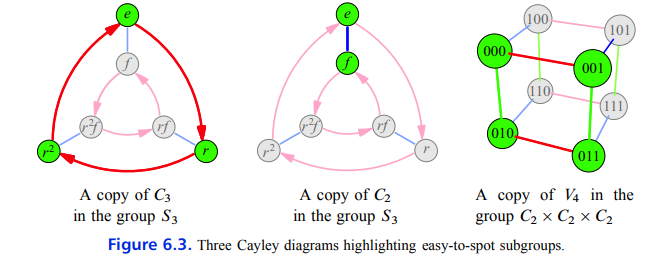
\includegraphics[scale=1]{cayleysubgroup}

\par
As shown in the image above, a subgroup is a subset of a group which retains a group structure under the same operation. For example, in the example on the left, we see a subset of the dihedral group (in this notation it is called $S_3$, whereas in Dummit \& Foote it would be denoted as $D_6$). We see that this subset of $D_6$ includes the elements generated by rotations of the polygon. Hence, we can see that this subset is closed under multiplication since $rr^2 = e = r^2r$, $rr = r^2$, $er = r = re$, and $r^2e = r^2 = er^2$. Lastly, we also have $ee = e$. In addition, we have shown that this subset is closed under inverses: $r = {r^2}^{-1}$, $r^2 = r^{-1}$, and $e = e^{-1}$. And finally, we see that $e$, the identity element, is contained in this subset. Thus, we can see that sometime of group structure has been retained here. Let us make this notion formal through the following definition \cite[\S 2.1, p. 46]{dummit}:

\par
\textbf{Definition} Let $G$ be a group. The subset $H$ of $G$ is a \textit{subgroup} of $G$ if $H$ is nonempty and $H$ is closed under products and inverses (i.e. $x, y \in H$ implies $x^{-1} \in H$ and $xy \in H$). If $H$ is a subgroup of $G$ we shall write $H \le G$.

\par
Note that $e \in H$ was not included here because it follows directly from the facts that $H$ is nonempty, closed under inverses, and closed under products. Since $H$ is nonempty, we have some element $a \in H$. Since $H$ is closed under inverses, we have $a^{-1} \in H$. And since $H$ is closed under products, we have $aa^{-1} = e \in H$ as required.

\par
Just as we condensed the subgroup criteria by removing the statement requiring the existence of $e$ in the group (since its existence is implied by the other properties), we can actually further condense the conditions that we need to check. In particular, we get the following proposition \cite[\S 2.1, p. 47]{dummit}:

\par
\textbf{Proposition 1.} (\textit{The Subgroup Criterion}) A subset $H$ of a group $G$ is a subgroup if and only if
\begin{enumerate}
\item $H \neq \emptyset$

\item for all $x, y \in H$, $xy^{-1} \in H$
\end{enumerate}

Furthermore, if $H$ is finite then it suffices to check that $H$ is nonempty and closed under multiplication.

\par
Hence, we can now show that a subset of a group $G$ is a subgroup if it satisfies just two properties -- it is nonempty and for every elements $x, y$ in the subset, we have $xy^{-1}$ in the subset as well.

\par
Now let us consider some specific families of subgroups \cite[\S 2.2, p. 49-50]]{dummit}:

\par
\textbf{Definitions:}
\begin{enumerate}

\item Define $C_G(A) = \{g \in G \ | \ gag^{-1} = a \ \text{for all} \ a \in A\}$. This subset of $G$ is called the \textit{centralizer} of $A$ in $G$. Since $gag^{-1} = a$ if and only if $ga = ag$, $C_G(A)$ is the set of elements of $G$ which commute with every element of $A$

\item Define $Z(G) = \{g \in G \ | \ gx = xg \ \text{for all} \ x \in G\}$, the set of elements commuting with all the elements of $G$. This subset of $G$ is called the \textit{center} of $G$

\item Define $gAg^{-1} = \{gag^{-1} \ | \ a \in A\}$. Define the \textit{normalizer} of $A$ in $G$ to be the set $N_G(A) = \{g \in G \ | \ gAg^{-1} = A\}$
\end{enumerate}

\par
These special subgroups will be quite important throughout our discussions of homomorphisms and quotient groups.

\subsection{Homomorphisms \& Isomorphisms}

\par
Now we turn our attention to functions between groups. We first start with homomorphisms, which describes a function from one group to another which maintains a portion of the group structure in some sense. The following image gives us an intuitive sense of what a homomorphism between groups can look like \cite{homomorphismwiki}:

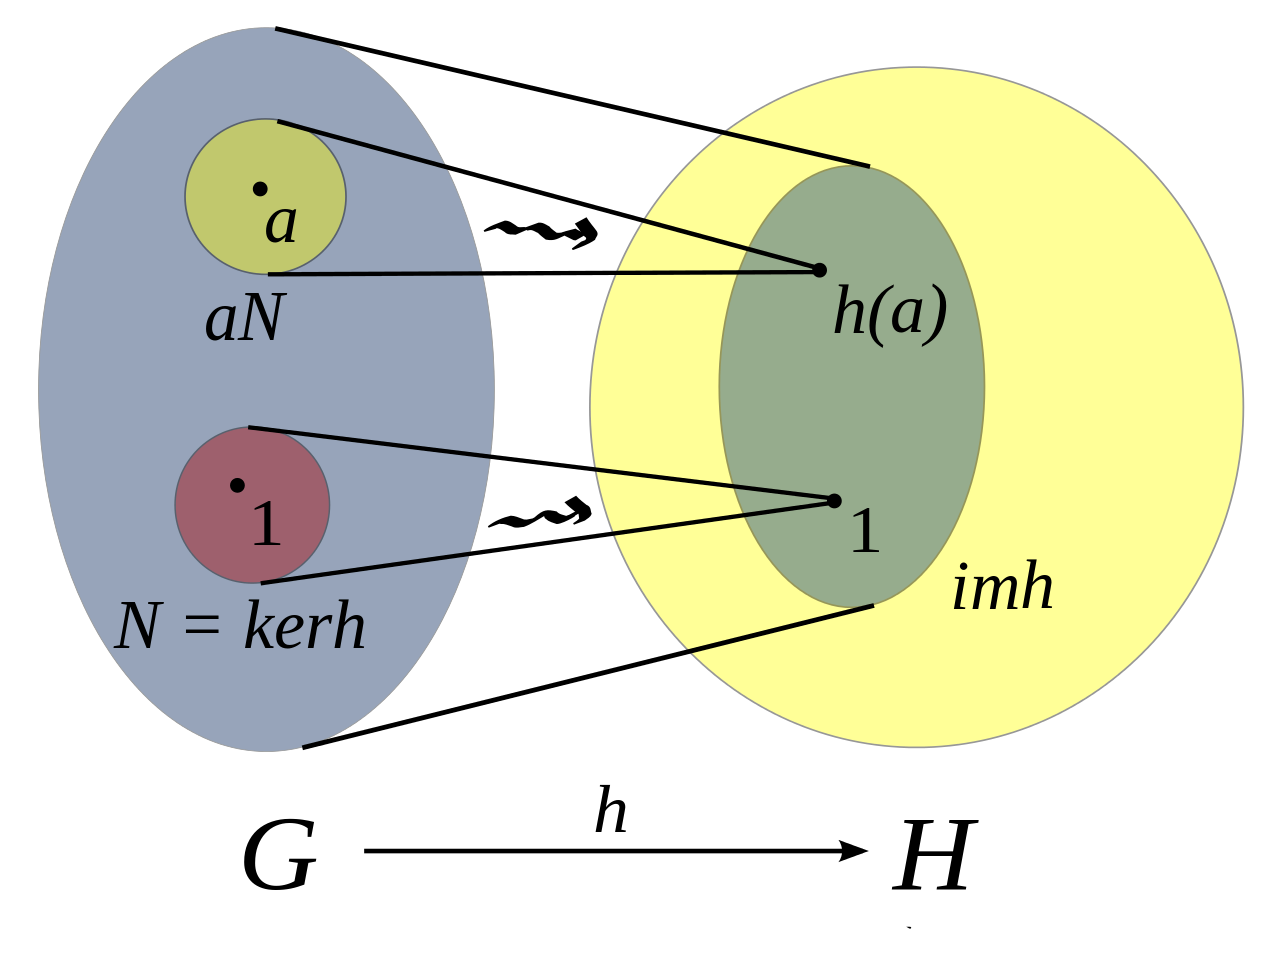
\includegraphics[scale=0.25]{homomorphism}

\par
As we can see, the above homomorphism maps elements of $G$ into elements of $H$. However, note that the image of the homomorphism $h$ in $H$ is a proper subset of $H$. That is, there are elements in $H$ which $h$ does not map any element of $G$ to. In addition, note that every element of $G$ in the circle around $a$ maps to $h(a)$ in $H$. In other words, multiple elements of $G$ can map to a single element of $H$ under a homomorphism $h$. These will be the key differences between homomorphisms and isomorphisms when we turn to defining these concepts rigorously.. We will give the following definition for a homomorphism \cite[\S 1.6, p. 36]]{dummit}:

\par
\textbf{Definition} Let $(G, *)$ and $(H, \diamond)$ be groups. A map $\varphi: G \to H$ such that 

\begin{align*}
\varphi(x * y) = \varphi(x) \diamond \varphi(y)
\end{align*}

is called a \textit{homomorphism}. We will usually omit the operation signs and write $\varphi(xy) = \varphi(x)\varphi(y)$, but remember that the operation on the left of the equation is not necessarily the same operation on the right of the equation.

\par
Hence, we can see that a homomorphism preserves the group operation in some sense -- the image of the product of $x$ and $y$ is the same as the product of the images of $x$ and $y$. Isomorphisms extend this group preservation in the following way \cite[\S 1.6, p. 37]{dummit}:

\par
\textbf{Definition} The map $\varphi: G \to H$ is called an \textit{isomorphism} and $G$ and $H$ are said to be \textit{isomorphic} or of the same \textit{isomorphism} type, written $G \cong H$, if
\begin{enumerate}
\item $\varphi$ is a homomorphism (i.e. $\varphi(xy) = \varphi(x)\varphi(y)$), and
\item $\varphi$ is a bijection
\end{enumerate}

\par
Thus, the homomorphism part of this definition ensures that the group operation is preserved (in the sense defined above), and the bijection part of the definition ensures that the groups $G$ and $H$ are the same size. Hence, two isomorphic groups can in some sense be considered the ``same'' group, just with potentially different names for the elements and operation.

\par
As we transition towards quotient groups, we must first discuss \textit{fibers} of homomorphisms. Let $\varphi: G \to H$ be a homomorphism and let $a \in H$. The \textit{fiber} of $\varphi$ over $a$ is the set of elements in $G$ which $\varphi$ maps to $a$. Hence, the kernel of $\varphi$ over $a$ is the same notion as the pre-image of $a$ under $\varphi$. We pay special attention to the fiber of $\varphi$ over $1$ (i.e. the identity element of $H$), which we call the \textit{kernel} of $\varphi$. We can define this formally as follows \cite[\S 3.1, p. 75]{dummit}:

\par
\textbf{Definition} If $\varphi$ is a homomorphism $\varphi: G \to H$, the \textit{kernel} of $\varphi$ is the set
\begin{align*}
\{g \in G \ | \ \varphi(g) = 1\}
\end{align*}

and will be denoted by $\ker \varphi$ (here $1$ is the identity of $H$).

\par
Equipped with this definition of the kernel of a homomorphism, we can now assert the following properties for a homomorphism \cite[\S 3.1, 75]{dummit}:

\textbf{Proposition 1.} Let $G$ and $H$ be groups and let $\varphi: G \to H$ be a homomorphism.
\begin{enumerate}
\item $\varphi(1_G) = 1_H$, where $1_G$ and $1_H$ are the identities of $G$ and $H$, respectively
\item $\varphi(g^{-1}) = \varphi(g)^{-1}$ for all $g \in G$
\item $\varphi(g^n) = \varphi(g)^n$ for all $n \in \ZZ$
\item $\ker \varphi$ is a subgroup of $G$
\item $\text{im}(\varphi)$, the image of $G$ under $\varphi$, is a subgroup of $H$
\end{enumerate}

\newpage
\subsection{Quotient Groups}

\par
Quotient groups extend the notion of division to groups. We can think about ``dividing'' a group into smaller groups and studying the relations between elements in this smaller group. We can see this notion visually in the following diagram \cite[\S 7.3, p. 133]{carter}:

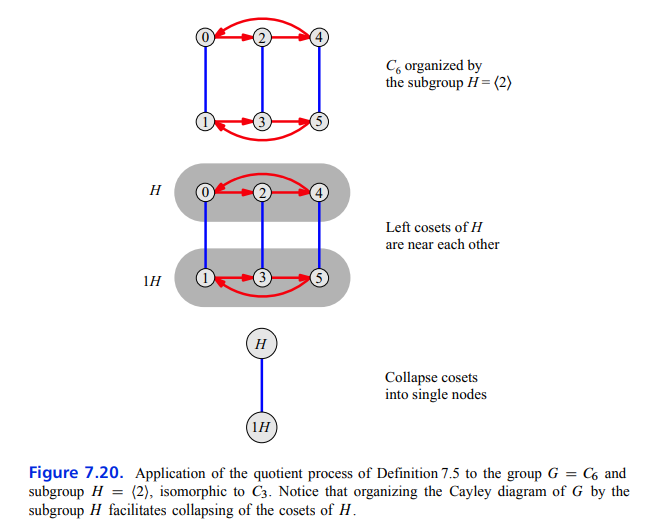
\includegraphics[scale=1]{quotient}

\par
We can see that $G$ is first divided up into two groups (called ``left cosets'', which we will discuss soon). Then, all elements contained within each coset are collapse into a single element. Lastly, we preserve the relationship between these two subgroups of $G$. Hidden within this intuitive sense of quotient groups is the fact that studying quotient groups and homomorphisms is actually equivalent \cite{dummit, quotientwiki}. We will see why in the following discussions,

\par
\textbf{Definition} Let $\varphi: G \to H$ be a homomorphism with kernel $K$. The \textit{quotient group} or \textit{factor group}, $G/K$ (read $G$ \textit{modulo} $K$ or simply $G$ \textit{mod} $K$), is the group whose elements are the fibers of $\varphi$ with group operation defined above: namely if $X$ is the fiber above $a$ and $Y$ is the fiber above $b$ then the product of $X$ with $Y$ is defined to be the fiber above the product $ab$.

\par
Hence, the group $G$ is divided into smaller subgroups (namely, the fibers of $\varphi$) by the kernel of $\varphi$. This connection between the kernel of $\varphi$ and its fibers over other elements will be captured by our work with cosets. Let us first define what a coset is \cite[\S 3.1, p. 77]{dummit}:

\par
\textbf{Definition} For any $N \le G$ and any $g \in G$ let
\begin{align*}
gN = \{gn \ | \ n \in N\} \;\; \text{and} \;\; Ng = \{ng \ | \ n \in N\}
\end{align*}

called respectively a \textit{left coset} and a \textit{right coset} of $N$ in $G$. Any element of a coset is called a \textit{representative} for the coset. 

\par
The relationship between this definition and the kernel of $\varphi$ is given by the following theorem \cite[\S 3.1, p. 77]{dummit}:

\par
\textbf{Theorem 3.} Let $G$ be a group and let $K$ be the kernel of some homomorphism from $G$ to another group. Then the set whose elements are the left cosets of $K$ in $G$ with operation defined by
\begin{align*}
uK \circ vK = (uv)K
\end{align*}

forms a group, $G/K$. In particular, this operation is well defined in the sense that if $u_1$ is any element in $uK$ and $v_1$ is any element in $vK$, then $u_1v_1 \in uvK$, i.e., $u_1v_1K = uvK$ so that the multiplication does not depend on the choice of representatives for the cosets. The same statement is true with ``right cosets'' in place of ``left cosets''.

\par
Hence, we can see from this theorem that the set of left cosets of $K$ is equivalent to the group $G/K$. We know that $G/K$ is the group whose elements are the fibers of $\varphi$, and so we must have that the left cosets of $K$ are equivalent to the fibers of $\varphi$. Hence, we see that we can actually ignore the fibers of $\varphi$ other than the kernel $K$ and simply take left cosets of $K$ in order to obtain the other fibers.

\subsection{More on Isomorphisms}

In this section, we detail some important theorems relating quotient groups and homomorphisms. These theorems are known as ``The Isomorphism Theorems'' and are central to the discussion of this section. The First Isomorphism Theorem is given by the following \cite[\S 3.3, p. 97]{dummit}:

\textbf{The First Isomorphism Theorem.} If $\varphi: G \to H$ is a homomorphism of groups, then $\text{ker} \varphi \normeq G$ and $G/\text{ker}\varphi \cong \varphi(G)$.

\par
The First Isomorphism Theorem allows us to assert that the kernel of a group homomorphism is a normal subgroup of the domain. This gives us the ability to discuss the quotient group $G/\text{ker}\varphi$, which we assert is congruent to the image of the domain under $\varphi$. The second isomorphism theorem is given by the following \cite[\S 3.3, p. 97]{dummit}:

\textbf{The Diamond Isomorphism Theorem.} Let $G$ be a group, let $A$ and $B$ be subgroups of $G$ and assume $A \leq N_G(B)$. Then $AB$ is a subgroup of $G$, $B \normeq AB$, $A \cap B \normeq A$, and $AB/B \cong A/A \cap B$.

\par
This is called The Diamond Isomorphism Theorem due to the section of the lattice of subgroups of $G$ that is considered. The final two isomorphism theorems are given as follows \cite[\S 3.3, p. 98-99]{dummit}:

\textbf{The Third Isomorphism Theorem.} Let $G$ be a group and let $H$ and $K$ be normal subgroups of $G$ with $H \leq K$. Then $K/H \normeq G/H$ and 
\begin{align*}
(G/H)/(K/H) \cong G/K.
\end{align*}

If we denote the quotient by $H$ with a bar, this can be written
\begin{align*}
\overline{G}/\overline{K} \cong G/K
\end{align*}

\textbf{The Lattice Isomorphism Theorem.} Let $G$ be a group and let $N$ be a normal subgroup of $G$. Then there is a bijection from the set of subgroups $A$ of $G$ which contain $N$ onto the set of subgroups $\overline{A} = A/N$ of $G/N$. In particular, every subgroup of $\overline{G}$ is of the form $A/N$ for some subgroup $A$ of $G$ containing $N$ (namely, its preimage in $G$ under the natural projection homomorphism from $G$ to $G/N$). This bijection has the following properties: for all $A, B \leq G$ with $N \leq A$ and $N \leq B$.
\begin{enumerate}
\item $A \leq B$ if and only if $\overline{A} \leq \overline{B}$
\item if $A \leq B$, then $|B : A| = |\overline{B} : \overline{A}|$
\item $\overline{\langle A, B \rangle} = \langle \overline{A}, \overline{B} \rangle$
\item $\overline{A \cap B} = \overline{A} \cap \overline{B}$
\item $A \normeq G$ if and only if $\overline{A} \normeq \overline{G}$
\end{enumerate}

The Third Isomorphism Theorem examines taking quotients of quotient groups, while The Lattice Isomorphism Theorem looks at the relationship between the lattice of subgroups of a quotient group (e.g. $G/N$) and the lattice of subgroups of the underlying group (e.g. $G$).

\subsection{Group Actions}

\par
As discussed in the introduction, group actions are when groups act upon sets. We define them as follows \cite[\S 1.7, p. 41]{dummit}:

\par
\textbf{Definition} A \textit{group action} of a group $G$ on a set $A$ is a map from $G \times A$ to $A$ (written as $g \cdot a$, for all $g \in G$ and $a \in A$) satisfying the following properties:
\begin{enumerate}
\item $g_1 \cdot (g_2 \cdot a) = (g_1g_2) \cdot a$ for all $g_1, g_2 \in G, a \in A$, and
\item $1 \cdot a = a$ for all $a \in A$
\end{enumerate}

We can extend these discussions of group actions using the language of homomorphisms as follows \cite[\S 4.1, p. 112]{dummit}:

\par
\textbf{Definition}
\begin{enumerate}
\item The \textit{kernel} of the action is the set of elements of $G$ that act trivially on every element of $A$: $\{g \in G \ | | g \cdot a = a \ \text{for all} \ a \in A\}$
\item For each $a \in A$, the \textit{stabilizer} of $a$ in $G$ is the set of elements of $G$ that fix the element $a$: $\{g \in G \ | \ g \cdot a = a\}$ and is denoted by $G_a$
\item An action is \textit{faithful} if its kernel is the identity
\end{enumerate}

\subsection{Direct and Semidirect Products}

Quotient groups allowed us to construct smaller groups from larger groups by ``removing'' unnecessary information. In this section, we will instead look at how to create larger groups from smaller groups through the use of direct and semidirect products. We will start by defining direct products in both the finite and countable cases \cite[\S 5.1, p. 152]{dummit}:

\par
\textbf{Definition.}
\begin{enumerate}
\item The \textit{direct product} $G_1 \times G_2 \times \cdots \times G_n$ of the groups $G_1, G_2, \ldots, G_n$ with operation $*_1, *_2, \ldots, *_n$, respectively, is the set of $n$-tuples $(g_1, g_2, \ldots, g_n)$ where $g_i \in G_i$ with operation defined componentwise:
\begin{align*}
(g_1, g_2, \ldots, g_n) * (h_1, h_2, \ldots, h_n) = (g_1 *_1 h_1, g_2 *_2 h_2, \ldots, g_n *_n h_n)
\end{align*}

\item Similarly, the \textit{direct product} $G_1 \times G_2 \times \cdots$ of the groups $G_1, G_2, \ldots$ with operations $*_1, *_2, \ldots$, respectively, is the set of sequences $(g_1, g_2, \ldots)$ where $g_i \in G_i$ with operation defined componentwise:
\begin{align*}
(g_1, g_2, \ldots) * (h_1, h_2, \ldots) = (g_1 * h_1, g_2 * h_2, \ldots)
\end{align*}
\end{enumerate}

The direct product of a set of groups actually preserves the information from each of the component groups. In fact, we can recover this information from the direct product group. The next proposition makes this notion formal \cite[\S 5.1, p. 154]{dummit}:

\newpage
\par
\textbf{Proposition 2.} Let $G_1, G_2, \ldots, G_n$ be groups and let $G = G_1 \times \cdots \times G_n$ be their direct product.
\begin{enumerate}
\item For each fixed $i$ the set of elements of $G$ which have the identity of $G_j$ in the $j^{\text{th}}$ position for all $j \neq i$ and arbitrary elements of $G_i$ in position $i$ is a subgroup of $G$ isomorphic to $G_i$:
\begin{align*}
G_i \cong \{(1, 1, \ldots, 1, g_i, 1, \ldots 1) \ | \ g_i \in G_i\},
\end{align*}

(here $g_i$ appears in the $i^{\text{th}}$ position). If we identify $G_i$ with this subgroup, then $G_i \normeq G$ and 
\begin{align*}
G/G_i \cong G_1 \times \cdots \times G_{i-1} \times G_{i+1} \times \cdots \times G_n
\end{align*}

\item For each fixed $i$ define $\pi_i: G \to G_i$ by
\begin{align*}
\pi_i((g_1, g_2, \ldots, g_n)) = g_i
\end{align*}

Then $\pi_i$ is a surjective homomorphism with
\begin{align*}
\text{ker}\pi_i &= \{(g_1, \ldots, g_{i-1}, 1, g_{i+1}, \ldots, g_n) \ | \ g_j \in G_j \text{ for all } j \neq i\}\\
&\cong G_1 \times \cdots \times G_{i-1} \times G_{i+1} \times \cdots \times G_n
\end{align*}
\end{enumerate}

We will now introduce the notion of a semidirect product, which generalizes direct products by relaxing the constraint that the constituent groups are normal. We start with the following theorem to set the stage \cite[\S 5.5, p. 176]{dummit}:

\par
\textbf{Theorem 10.} Let $H$ and $K$ be groups and let $\varphi$ be a homomorphism from $K$ into $\text{Aut}(H)$. Let $\cdot$ denote the (left) action of $K$ on $H$ determined by $\varphi$. Let $G$ be the set of ordered pairs $(h, k)$ with $h \in H$ and $k \in K$ and define the following multiplication on $G$:
\begin{align*}
(h_1, k_1)(h_2, k_2) = (h_1 k_1 \cdot h_2, k_1k_2)
\end{align*}

\begin{enumerate}
\item This multiplication makes $G$ into a group of order $|G| = |H||K|$
\item The sets $\{(h, 1) \ | \ h \in H\}$ and $\{(1, k) \ | \ k \in K\}$ are subgroups of $G$ and the maps $h \mapsto (h, 1)$ for $h \in H$ and $k \mapsto (1, k)$ for $k \in K$ are isomorphisms of these subgroups with the groups $H$ and $K$ respectively:
\begin{align*}
H \cong \{(h, 1) \ | \ h \in H\} \text{  and  } K \cong \{(1, k) \ | \ k \in K \}
\end{align*}
\end{enumerate}

Identifying $H$ and $K$ with their isomorphic copies in $G$ described in (2) we have
\begin{enumerate}
\setcounter{enumi}{2}

\item $H \normeq G$
\item $H \cap K = 1$
\item for all $h \in H$ and $k \in K$, $khk^{-1} = k \cdot h = \varphi(k)(h)$
\end{enumerate}

Equipped with this background information, we can now precisely define what a semidirect product is \cite[\S 5.5, p. 177]{dummit}:

\par
\textbf{Definition.} Let $H$ and $K$ be groups and let $\varphi$ be a homomorphism from $K$ into $\text{Aut}(H)$. The group described in Theorem 10 is called the \textit{semidirect product} of $H$ and $K$ with respect to $\varphi$ and will be denoted by $H \rtimes_{\varphi} K$ (when there is no danger of confusion we shall simply write $H \rtimes K$).

\par
The following proposition and theorem provide us with useful tools for working with semidirect products \cite[\S 5.5, p. 177, 180]{dummit}:

\par
\textbf{Proposition 11.} Let $H$ and $K$ be groups and let $\varphi: K \to \text{Aut}(H)$ be a homomorphism. Then the following are equivalent:
\begin{enumerate}
\item the identity (set) map between $H \rtimes K$ and $H \times K$ is a group homomorphism (hence an isomorphism)
\item $\varphi$ is the trivial homomorphism from $K$ into $\text{Aut}(H)$
\item $K \normeq H \rtimes K$
\end{enumerate}

\par
\textbf{Theorem 12.} Suppose $G$ is a group with subgroups $H$ and $K$ such that
\begin{enumerate}
\item $H \normeq G$
\item $H \cap K = 1$
\end{enumerate}

Let $\varphi: K \to \text{Aut}(H)$ be the homomorphism defined by mapping $k \in K$ to the automorphism of left conjugation by $k$ on $H$. Then $HK \cong H \rtimes K$. In particular, if $G = HK$ with $H$ and $K$ satisfying $(1)$ and $(2)$, then $G$ is the semidirect product of $H$ and $K$.

\subsection{Rings}

We now extend our study of groups to a new algebraic structure: rings. Rings are a central theme throughout many fields of algebra which include many of the same notions that we studied in groups with a few key differences. Whereas groups consisted of a set with one binary operation, rings are a set with two binary operations. Moreover, these binary operations must interact with each other in some sense, otherwise we would consider them as two different groups. We can formalize this notion with the following definition \cite[\S 7.1, p. 223]{dummit}:

\par
\textbf{Definition.}
\begin{enumerate}
\item A \textit{ring} $R$ is a set together with two binary operations $+$ and $\times$ (called addition and multiplication) satisfying the following axioms:
\begin{enumerate}[label=(\roman*)]

\item $(R, +)$ is an \textit{abelian} group

\item $\times$ is associative: $(a \times b) \times c = a \times (b \times c)$ for all $a, b, c \in R$

\item the \textit{distributive laws} hold in $R$: for all $a, b, c \in R$
\begin{align*}
(a + b) \times c = (a \times c) + (b \times c) \text{  and  } a \times (b + c) = (a \times b) + (a \times c)
\end{align*}
\end{enumerate}

\item The ring $R$ us \textit{commutative} if multiplication is commutative.

\item The ring $R$ is said to have an \textit{identity} (or \textit{contain a} 1) if there is an element $1 \in R$ with
\begin{align*}
1 \times a = a \times 1 = a \text{  for all } a \in R
\end{align*}
\end{enumerate}

Rings can be further classified based off certain attributes, such as the following \cite[\S 7.1, p. 224]{dummit}:

\par
\textbf{Definition.} A ring $R$ with identity $1$, where $1 \neq 0$, is called a \textit{division ring} (or \textit{skew field}) if every nonzero element $a \in R$ has a multiplicative inverse, i.e., there exists $b \in R$ such that $ab = ba = 1$. A commutative division ring is called a \textit{field}.

\par
Commutative division rings (or fields) are extremely common throughout undergrad mathematics. For example, the real numbers and the integers equipped with our usual notions of multiplication and addition are two examples of fields.

\par
The following proposition gives us some properties of rings \cite[\S 7.1, p. 236]{dummit}:

\par
\textbf{Proposition 1.} Let $R$ be a ring. Then
\begin{enumerate}
\item $0a = a0 = 0$ for all $a \in R$
\item $(-a)b = a(-b) = -(ab)$ for all $a, b \in R$ (recall $-a$ is the additive inverse of $a$)
\item $(-a)(-b) = ab$ for all $a, b \in R$
\item if $R$ has an identity $1$, then the identity is unique and $-a = (-1)a$
\end{enumerate}

Hence, we can see that rings retain some the usual operations that we have seen for addition and multiplication in our more typical settings, such as the real numbers. 

\par
\textbf{Definition.} Let $R$ be a ring.
\begin{enumerate}
\item A nonzero element $a$ of $R$ is called a \textit{zero divisor} if there is a nonzero element $b$ in $R$ such that either $ab = 0$ or $ba = 0$

\item Assume $R$ has an identity $1 \neq 0$. An element $u$ of $R$ is called a \textit{unit} in $R$ if there is some $v$ in $R$ such that $uv = vu = 1$. The set of units in $R$ is denoted $R^{\times}$. 
\end{enumerate}

The units in $R$ form a group under multiplication. Rings that share certain characteristics with $\ZZ$ are defined as follows:

\par
\textbf{Definition.} A commutative ring with identity $1 \neq 0$ is called an \textit{integral domain} if it has no zero divisors.

\par
\textbf{Proposition 2.} Assume $a, b$ and $c$ are elements of any ring with $a$ not a zero divisior. If $ab = ac$, then either $a = 0$ or $b = c$ (i.e., if $a \neq 0$ we can cancel the $a$'s). In particular, if $a, b, c$ are any elements in an integral domain and $ab = ac$, then either $a = 0$ or $b = c$.

\par
\textbf{Corollary 3.} Any finite integral domain is a field.

\par
Now, similarly to groups and subgroups, we can define a subset of a ring which retains the structure of the parent ring. We can make this notion formal through the following definition \cite[\S 7.1, p. 228]{dummit}:

\par
\textbf{Definition.} A \textit{subring} of the ring $R$ is a subgroup of $R$ that is closed under multiplication.

\subsection{Ring Homomorphisms and Quotient Rings}

Ring homomorphisms are very similar in concept to group homomorphisms. However, in the case of rings, homomorphisms must retain both the additive and multiplicative structure of the domain ring. We can see this in the following definition \cite[\S 7.3, p. 239]{dummit}:

\par
\textbf{Definition.} Let $R$ and $S$ be rings.
\begin{enumerate}
\item A \textit{ring homomorphism} is a map $\varphi: R \to S$ satisfying
\begin{enumerate}[label=(\roman*)]

\item $\varphi(a + b) = \varphi(a) + \varphi(b)$ for all $a, b \in R$ (so $\varphi$ is a group homomorphism on the additive groups) 

\item $\varphi(ab) = \varphi(a)\varphi(b)$ for all $a, b \in R$
\end{enumerate}

\item The \textit{kernel} of the ring homomorphism $\varphi$, denoted $\text{ker}\phi$, is the set of elements of $R$ that map to $0$ in $S$ (i.e., the kernel of $\varphi$ viewed as a homomorphism of additive groups).

\item A bijective ring homomorphism is called an \textit{isomorphism}.

\end{enumerate}

Again, similarly to the case of group homomorphisms, we can relate the image of a ring homomorphism to its codomain \cite[\S 7.3, p. 239]{dummit}:
\par
\textbf{Proposition 5.} Let $R$ and $S$ be rings and let $\varphi: R \to S$ be a homomorphism.
\begin{enumerate}
\item The image of $\varphi$ is a subring of $S$.

\item The kernel of $\varphi$ is a subring of $R$. Furthermore, if $\alpha \in \text{ker}\varphi$ then $r\alpha$ and $\alpha r \in \text{ker} \varphi$ for every $r \in R$, i.e., $\text{ker} \varphi$ is closed under multiplication by elements from $R$.

\end{enumerate}

Naturally, we can wonder if an analogue of normal subgroups (and by extension quotient groups) exists in the ring setting. The concept related to normal subgroups is called an ideal and is conceptualized as a subset of a ring $R$ which is closed under multiplication on the left and on the right by elements from $R$. Making this definition formal yields \cite[\S 7.3, p. 242]{dummit}:

\par
\textbf{Definition.} Let $R$ be a ring, let $I$ be a subset of $R$ and let $r \in R$.
\begin{enumerate}
\item $rI = \{ra \ | \ a \in I\} \text{  and  } Ir = \{ar \ | \ a \in I\}$

\item A subset $I$ of $R$ is a \textit{left ideal} of $R$ if
\begin{enumerate}[label=(\roman*)]

\item $I$ is a subring of $R$

\item $I$ is closed under left multiplication by elements from $R$, i.e., $rI \subset I$ for all $r \in R$

Similarly, $I$ is a \textit{right ideal} if (i) holds and in place of (ii) one has
\item $I$ is closed under right multiplication by elements from $R$, i.e., $Ir \subset I$ for all $r \in R$
\end{enumerate}

\item A subset $I$ that is both a left ideal and a right ideal is called an \textit{ideal} (or, for added emphasis, a \textit{two-sided ideal}) of $R$
\end{enumerate}

Now we will define operations on quotient rings \cite[\S 7.3, p. 242-243]{dummit}:

\par
\textbf{Proposition 6.} Let $R$ be a ring and let $I$ be an ideal of $R$. Then the (additive) quotient group $R/I$ is a ring under the binary operation:
\begin{align*}
(r+I) + (s+I) = (r+s) + I \text{  and  } (r+I) \times (s+I) = (rs) + I
\end{align*}

for all $r, s \in R$. Conversely, if $I$ is any subgroup such that the above operations are well defined, then $I$ is an ideal of $R$.

\par
\textbf{Definition:} When $I$ is an ideal of $R$, the ring $R/I$ with the operations in the previous proposition is called the \textit{quotient ring} of $R$ by $I$.

\par
Thus, we now have a formal notion of normal subgroups and quotient groups in the ring context. In keeping with the theme of extending group concepts to rings, we can now discuss the Isomorphism Theorems as they apply to rings \cite[\S 7.3, p. 243, 246]{dummit}:

\textbf{Theorem 7 \& 8}
\begin{enumerate}
\item \textit{(The First Isomorphism Theorem for Rings)} If $\varphi: R \to S$ is a homomorphism of rings, then the kernel of $\varphi$ is an ideal of $R$, the image of $\varphi$ is a subring of $S$ and $R/\text{ker}\varphi$ is isomorphic as a ring to $\varphi(R)$.
\item If $I$ is any ideal of $R$, then the map
\begin{align*}
R \to R/I \text{   defined by   } r \mapsto r + I
\end{align*}

is a surjective ring homomorphism with kernel $I$ (this homomorphism is called the \textit{natural projection} of $R$ onto $R/I$). Thus every ideal is the kernel of a ring homomorphism and vice versa.

\item \textit{(The Second Isomorphism Theorem for Rings)} Let $A$ be a subring and let $B$ be an ideal of $R$. Then $A + B = \{a+b \ | \ a \in A, b \in B\}$ is a subring of $R$, $A \cap B$ is an ideal of $A$ and $(A+B)/B \cong A/(A \cap B)$

\item \textit{(The Third Isomorphism Theorem for Rings)} Let $I$ and $J$ be ideals of $R$ with $I \subset J$. Then $J/I$ is an ideal of $R/I$ and $(R/I)/(J/I) \cong R/J$.

\item \textit{(The Fourth or Lattice Isomorphism Theorem for Rings)} Let $I$ be an ideal of $R$. The correspondence $A \leftrightarrow A/I$ is an inclusion preserving bijection between the set of subrings $A$ of $R$ that contain $I$ and the set of subrings of $R/I$. Furthermore, $A$ (a subring containing $I$) is an ideal of $R$ if and only if $A/I$ is an ideal of $R/I$.
\end{enumerate}

\subsection{Properties of Ideals}

In this section, we will now expand on the properties of ideals. We will begin with discussing ideals generated by an element or a set of elements, just as we have seen in the case of groups. The definition is as follows \cite[\S 7.4, p. 251]{dummit}:

\par
\textbf{Definition.} Let $A$ be any subset of the ring $R$.
\begin{enumerate}
\item Let $(A)$ denote the smallest ideal of $R$ containing $A$, called \textit{the ideal generated by A}
\item Let $RA$ denote the set of all finite sums of elements of the form $ra$ with $r \in R$ and $a \in A$ i.e., $RA = \{r_1a_1 + a_2r_2 + \cdots a_nr_n \ | \ r_i \in R, a_i \in An n \in \ZZ^+\}$ and $RAR = \{r_1a_1r_1' + r_2a_2r_2' + \cdots + r_na_nr_n' \ | \ r_i, r_i' \in R, a_i \in A, n \in \ZZ^+\}$
\item An ideal generated by a single element is called a \textit{principal ideal}.
\item An ideal generated by a finite set is called a \textit{finitely generated ideal}.
\end{enumerate}

Note that if $R$ is commutative, then $RA = AR = RAR = (A)$. An element $b \in R$ belongs to an ideal $(a)$ if and only if $b = ra$ for some $r \in R$. In other words, $b$ is an element of $(a)$ if and only if $b$ is a multiple of $a$. It can now be useful to discuss the units of an ideal \cite[\S 7.4, p. 253]{dummit}:

\par
\textbf{Proposition 9.} Let $I$ be an ideal of $R$.
\begin{enumerate}
\item $I = R$ if and only if $I$ contains a unit.
\item Assume $R$ is commutative. Then $R$ is a field if and only if its only ideals are $0$ and $R$.
\end{enumerate}

The ideals of a ring can be ordered in such a way that we can find a ``largest'' ideal within the ring \cite[\S 7.4, p. 253-254]{dummit}:

\par
\textbf{Definition.} An ideal $M$ in an arbitrary ring $S$ is called a \textit{maximal ideal} if $M \neq S$ and the only ideals containing $M$ are $M$ and $S$.

\par
\textbf{Proposition 11.} In a ring with identity every proper ideal is contained in a maximal ideal.

\par
\textbf{Proposition 12.} Assume $R$ is commutative. The ideal $M$ is a maximal ideal if and only if the quotient ring $R/M$ is a field.

\par
Lastly, we can discuss prime ideals, which give an extension to the notion of closure under multiplication for ideals \cite[\S 7.4, p. 255-256]{dummit}:

\par
\textbf{Definition.} Assume $R$ is commutative. An ideal $P$ is called a \textit{prime ideal} if $P \neq R$ and whenever the product $ab$ of two elements $a, b \in R$ is an element of $P$, then at least one of $a$ and $b$ is an element of $P$.

\par
\textbf{Proposition 13.} Assume $R$ is commutative. Then the ideal $P$ is a prime ideal in $R$ if and only if the quotient ring $R/P$ is an integral domain.

\par
\textbf{Corollary 14.} Assume $R$ is commutative. Every maximal ideal of $R$ is a prime ideal.

\newpage
\subsection{Euclidean Domains and Principal Ideal Domains}

In this section, we examine more specialized types of rings, beginning with rings with a division algorithm. These rings are known as Euclidean Domain. In order to discuss Euclidean Domains, we must first define the idea of a norm on an integral domain $R$ \cite[\S 8.1, p.  270]{dummit}:

\par
\textbf{Definition.} Any function $N: R \to \ZZ^+ \cup \{0\}$ with $N(0) = 0$ is called a \textit{norm} on the integral domain $R$. If $N(a) > 0$ for $a \neq 0$ define $N$ to be a \textit{positive norm}.

\par
Equipped with this definition of a norm, we can now defined Euclidean Domains \cite[\S 8.1, p. 270]{dummit}:

\par
\textbf{Definition.} The integral domain $R$ is said to be a \textit{Euclidean Domain} (or possess a \textit{Division Algorithm}) if there is a norm $N$ on $R$ such that for any two elements $a$ and $b$ of $R$ with $b \neq 0$ there exist elements $q$ and $r$ in $R$ with
\begin{align*}
a = qb + r \text{   with } r = 0 \text{ or } N(r) < N(b)
\end{align*}

The element $q$ is called the \textit{quotient} and the element $r$ the \textit{remainder} of the division.

\par
The key point here is that Euclidean Domains allow us to make use of the \textit{Euclidean Algorithm}, which furnishes us with a method for finding the greatest common divisor of two elements. It is now important to discuss the ideals of Euclidean Domains \cite[\S 8.1, p. 273]{dummit}:

\par
\textbf{Proposition 1.} Every ideal in a Euclidean Domain is principal. More precisely, if $I$ is any nonzero ideal in the Euclidean Domain $R$, then $I = (d)$, where $d$ is any nonzero element of $I$ of minimum norm.

\par
We will now define the second main type of rings, the Principal Ideal Domain \cite[\S 8.2, p. 279]{dummit}:

\textbf{Definition.} A \textit{Principal Ideal Domain} (P.I.D) is an integral domain in which every ideal is principal.

\section{Conclusion}

\par
This first pass into the modern form of Algebra has been enlightening, generalizing a subject which I thought I was intimately familiar with. The notions of groups, quotient groups, isomomorphisms, and more are extremely powerful, and I see them often in other mathematical contexts. For example, in Dynamics, we talk about the order of elements under a specific iterated map. This is akin to our discussion of the order of elements within a group. However, with the increased abstractedness and power of the theorems in Modern Algebra when compared with Classical Algebra, I feel that I have lost some intuition for the objects that we are working with. It is my hope that the historical context given in the main introduction as well as the informal introductions \& pictures at the start of each topic will help me and potentially others to build more intuition for and understanding of the subject.

\newpage
\begin{thebibliography}{9}

\bibitem{dummit}
Dummit, David Steven., and Richard M. Foote. \textit{Abstract Algebra}. 3rd ed., John Wiley \& Sons, 2004. 

\bibitem{pinter}
Pinter, Charles C. \textit{A Book of Abstract Algebra}. 2nd ed., Dover Publications, 2013. 

\bibitem{carter}
Carter, Nathan C. \textit{Visual Group Theory}. The Mathematical Association of America, 2009. 

\bibitem{schaum}
Ayres, Frank, and Lloyd R Jaisingh. \textit{Schaum's Outlines: Abstract Algebra}. 2nd ed., McGraw-Hill, 1971. 

\bibitem{algebrawiki}
“Algebra.” \textit{Wikipedia}, Wikimedia Foundation, 16 Oct. 2020, \texttt{en.wikipedia.org/wiki/Algebra}. 

\bibitem{abstractwiki}
“Abstract Algebra.” \textit{Wikipedia}, Wikimedia Foundation, 19 Sept. 2020,\\ \texttt{en.wikipedia.org/wiki/Abstract\_algebra}. 

\bibitem{groupwiki}
“Group (Mathematics).” \textit{Wikipedia}, Wikimedia Foundation, 17 Oct. 2020,\\ \texttt{en.wikipedia.org/wiki/Group\_(mathematics)}.

\bibitem{subgroupwiki}
“Subgroup.” \textit{Wikipedia}, Wikimedia Foundation, 14 June 2020, \texttt{en.wikipedia.org/wiki/Subgroup}. 

\bibitem{homomorphismwiki}
“Group Homomorphism.” \textit{Wikipedia}, Wikimedia Foundation, 1 Oct. 2020,\\ \texttt{en.wikipedia.org/wiki/Group\_homomorphism}.  

\bibitem{quotientwiki}
“Quotient Group.” \textit{Wikipedia}, Wikimedia Foundation, 1 Oct. 2020,\\ \texttt{https://en.wikipedia.org/wiki/Quotient\_group}. 

\bibitem{dihedralwiki} 
Dihedral Group.” \textit{Wikipedia}, Wikimedia Foundation, 1 Oct. 2020,\\ \texttt{https://en.wikipedia.org/wiki/Dihedral\_group}. 
\end{thebibliography}

\end{document}